\documentclass[10pt,twocolumn]{article}

% Builds with plain pdflatex (no conference style files needed).
\usepackage[margin=0.75in]{geometry}
\usepackage{booktabs}
\usepackage{amsmath}
\usepackage{amssymb}
\usepackage{amstext}
\usepackage{graphicx}
\graphicspath{{figures/}}
\usepackage[hidelinks]{hyperref}
\usepackage{caption}
\captionsetup{font=footnotesize,skip=3pt}
\usepackage{titlesec}
\titlespacing*{\section}{0pt}{7pt plus 2pt minus 2pt}{3pt}
\setlength{\textfloatsep}{7pt plus 2pt minus 2pt}
\setlength{\floatsep}{5pt plus 2pt minus 2pt}

\newcommand{\uu}[1]{\,\textsf{#1}}

\title{\vspace{-2em}\bfseries OS Noise for Agentic AI:\\
A Kernel-Trace Study of How Container Resource Limits\\
Slow Down and Break AI Coding Agents}

\author{Yuvraj Sehgal \quad Naser Ezzati-Jivan\\
\small Department of Computer Science, Brock University}
\date{}

\begin{document}
\maketitle

\begin{abstract}
When a coding agent is slow, the usual diagnosis is the language model. But
agents run inside containers, and containers come with resource limits (a
fractional CPU, a memory ceiling, an I/O budget) set by whatever platform
runs them. We ask how much of an agent's wall-clock time these limits
silently take. We answer with kernel tracing (LTTng) on two production
agents, \emph{Claude Code} and \emph{Codex CLI}, across 260 controlled runs.

On a well-provisioned machine the agent is ${\approx}84\%$ LLM-bound. This
is a regime, not a law. As resources tighten, the agent does not do less
work; it waits (up to $4.7\times$ longer in the stressed phase) or a process
is OOM-killed mid-task. Over-subscribing cores inflates a parallel phase by
nearly $300\%$ along a textbook queueing law, and a hard memory limit below
a process's footprint is a sharp, reproducible cliff. Every effect
reproduces across both agents and agrees with the cgroup's own counters.
Which limit bites depends on the workload: a lightweight coding task is
slowed only by the CPU cap and killed only when memory falls below the
agent's own footprint. When an agent feels slow, look at the
resources it was given, not only the model.
\end{abstract}

\section{Introduction}

When an agentic workflow is slow, practitioners reach for the model: a
bigger context, a faster endpoint, fewer tokens. This paper measures a cost
that view cannot see. Agent harnesses such as Codex CLI and Claude Code run
their tool calls inside containers and sandboxes. The platform that hosts
them (CI runners, Kubernetes pods, shared build machines) routinely gives
those containers resource limits: a fractional CPU, a memory ceiling, an I/O
budget. We ask: \emph{how much latency does the operating system, under such
a limit, add on top of the LLM?}

On a well-provisioned machine an agent is overwhelmingly LLM-bound. It
spends most of its wall time blocked on the network, waiting for the model.
But each resource limit has a threshold. Past it, that limit, not the model,
decides how long the agent takes, or whether it finishes at all. We make
this precise with kernel traces, which see the mechanism (scheduler, memory
reclaim, block layer) that application-level metrics cannot. Our
contributions are:
\begin{itemize}\itemsep0pt
  \item A reproducible, kernel-only method for measuring agentic workloads
  (a fixed task, a cgroup, an LTTng trace, and the cgroup's own counters as
  ground truth), with a trace-based finding that the agent is
  ${\approx}84\%$ LLM-bound by default.
  \item A catalogue of four \emph{configuration-level} mechanisms of OS
  noise (CPU cap, core over-subscription, memory cap, disk-I/O cap), each
  with a predicted effect the data confirms and the range in which its
  threshold falls.
  \item An end-to-end test on a realistic coding task showing \emph{which}
  mechanisms a lightweight agent actually trips, and validation of every
  effect on two unrelated agents.
\end{itemize}

\section{Related Work}

Operating-system noise (``OS jitter'') is a long-studied source of
performance variability in HPC and benchmarking, where background kernel
activity perturbs an otherwise CPU-bound job; recent work has carried the
idea to user-facing settings such as web-browser benchmarking. We transfer
the lens to LLM-driven coding agents and study noise that is \emph{imposed
by configuration} (cgroup limits) rather than ambient. To our knowledge this
is the first kernel-trace characterization of how container resource limits
affect agentic AI latency and reliability.

\section{Methodology}
\label{sec:method}

Every run executes on one fixed Google Cloud VM (Table~\ref{tab:setup}), so
the resource limit under test is the only thing that varies. On it we study
two independent production agents. They share no code: one is a Node
process, the other a Rust/tokio binary, and they reach different models over
different APIs. Running both lets us separate properties of agentic
workloads from artifacts of a single harness.

\begin{table}[t]
  \centering
  \footnotesize
  \setlength{\tabcolsep}{3pt}
  \begin{tabular}{@{}l p{0.78\columnwidth}@{}}
    \toprule
    \multicolumn{2}{@{}l}{\textbf{Machine} (Google Cloud \texttt{n2-standard-4})} \\
    \midrule
    CPU     & Intel Xeon 2.80\,GHz, 4 vCPUs (2 cores, 2 SMT each) \\
    Memory  & 15\,GiB, no swap \\
    Disk    & \texttt{pd-balanced}, ${\approx}205$\uu{MB/s} seq.\ read \\
    OS      & Ubuntu 24.04.5, kernel \texttt{7.0.0-1011-gcp} \\
    Tracing & LTTng 2.15.3, Babeltrace2 \\
    \midrule
    \multicolumn{2}{@{}l}{\textbf{Agents} (headless)} \\
    \midrule
    Claude Code & v2.1.296, Claude Opus 5.5, \texttt{claude -p} \\
    Codex CLI   & v0.162.1, \texttt{gpt-6-luna} (OpenRouter), \texttt{codex exec} \\
    \bottomrule
  \end{tabular}
  \caption{Experimental setup. All numbers come from this one VM.}
  \label{tab:setup}
\end{table}

\emph{Tasks.} Each run hands the agent one small, self-contained coding task
in a throwaway Git repository. A \emph{bug-fix} task provides a few short
Python modules with seeded bugs and a test suite; the agent must fix the bugs
until the tests pass. An \emph{implementation} task provides function stubs
with docstring specifications and a test suite; the agent must write the
code that satisfies them. For Problems~2--4 the agent simply launches a
fixed, instrumented workload (parallel CPU workers, or a large file read),
so the measured work is identical from run to run. In every case the
repository is regenerated byte-for-byte, the prompt is fixed, the session is
fresh, and an integrity check confirms the agent never edited the protected
test file.

\emph{Resource limits and protocol.} The agent and all of its tool
subprocesses run inside a dedicated cgroup~v2 group, recreated for each run
so its counters start at zero. Each run imposes exactly one limit, a CPU-bandwidth cap
(\texttt{cpu.max}), a memory cap (\texttt{memory.high} or
\texttt{memory.max}), or a disk-I/O cap (\texttt{io.max}), swept from
generous to tight. Core over-subscription
(Problem~2) is the one exception: it uses no cgroup limit and simply places
more runnable threads in the group than the machine has cores. Every
condition is run five times (three for purely observational cells) in
random order, and we report medians, so LLM nondeterminism and time-of-day
effects cannot line up with any one condition. For the three stress
experiments (cores, memory, disk) we pre-registered the predicted direction
of each effect before collecting data.

\begin{figure}[t]\centering
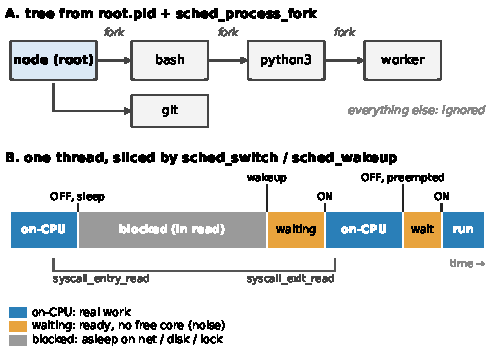
\includegraphics[width=\columnwidth]{fig_method}
\caption{From trace to time accounting. (A) The process tree is rebuilt
by following every \texttt{sched\_process\_fork} from \texttt{root.pid}.
(B) at a switch, \texttt{prev\_state}${=}0$ or the preempt flag (${=}256$ on
this kernel) means the thread still wants a core (waiting); any other value
means asleep (blocked); a wakeup moves blocked to waiting. The
system call the thread is inside tags its blocked time.}
\label{fig:method}
\end{figure}

\emph{Tracing and analysis.} Without modifying the agent, we record a
curated kernel LTTng profile: all system calls plus the scheduler,
block-layer, networking, interrupt, power, and memory-reclaim
(\texttt{mm\_vmscan}) tracepoints, each event tagged with its process and
thread. We rebuild the agent's process tree (Figure~\ref{fig:method}) from \texttt{root.pid} via
\texttt{sched\_process\_fork}, so every spawned tool is captured, and a
per-thread state machine labels every slice of a thread's time as
\emph{on-CPU}, \emph{runnable-but-waiting} (CPU ``noise''), or
\emph{blocked} on a named system call. We never trust the trace alone: we
also snapshot the cgroup's own accounting (\texttt{cpu.stat},
\texttt{memory.*}, \texttt{io.stat}) as an independent ground truth.
On-CPU time from the trace agrees with \texttt{cpu.stat} usage to a few
percent on throttled runs (median ${\approx}2\%$), loosening to
${\approx}18\%$ on unthrottled runs where many short-lived helper threads are
mapped late; the throttle figures we report come straight from
\texttt{cpu.stat}, so a gross parsing error would surface at once.

\emph{Baseline: how much of a run is the model?} From the trace we identify
the API sockets (the file descriptors the agent \texttt{connect}s to on port
443) and measure, per request, the interval from the request write to the
last streamed response read. The union of these intervals is the time a
model request is outstanding. On an unthrottled machine the agent spends a
median of \textbf{84\%} of wall-clock time with a request in flight
(80--91\% across ten runs, two tasks) and only ${\approx}4.7$ CPU-seconds
computing locally. Tightening the CPU cap does not change how long the
model takes; it adds throttle wait, so the model's share falls to
${\approx}53\%$ at a quarter core. No timing counter
can produce this split; only the trace can attribute time per descriptor.

\section{Problem 1: CPU Cap}
\label{sec:cpu}

We cap the agent's cgroup with \texttt{cpu.max} at unlimited, 1, 0.5, and
0.25 core, for two tasks (bug-fix, implement), 5 reps each (40 runs). The
agent's compute demand is fixed at roughly 4--5 CPU-seconds, whatever the
cap. The cap does not reduce the work; it turns compute into \emph{throttle
wait}. Table~\ref{tab:cpu} shows both tasks: on-CPU time is flat while
throttled time and wall time climb as the cap tightens. At 1 core the agent
is still LLM-bound. At 0.5 core and below the cap substantially increases
execution time. At 0.25 core throttle reaches 61\% of the implement run,
though the model still accounts for roughly half of the wall clock, so the limit is a major component rather than the
sole bottleneck.

\begin{table}[t]\centering\footnotesize
\setlength{\tabcolsep}{4pt}
\caption{Problem~1, medians over $n{=}5$. On-CPU demand is flat across
caps; the cap converts it into throttle wait. ``thr.'' is throttled time in
seconds and as a fraction of wall.}
\label{tab:cpu}
\begin{tabular}{@{}lrrrrr@{}}
\toprule
\texttt{cpu.max} & wall (s) & $\Delta$wall & on-CPU (s) & thr.\ (s) & thr.\ \% \\
\midrule
\multicolumn{6}{@{}l}{\textit{bug-fix}} \\
unlimited & 23.4 & --     & 4.4 & 0.0  & 0 \\
1 core    & 24.4 & $+4$\%  & 3.7 & 0.3  & 1 \\
0.5 core  & 22.4 & $-4$\%  & 3.7 & 4.4  & 20 \\
0.25 core & 28.9 & $+24$\% & 3.9 & 13.7 & 47 \\
\addlinespace
\multicolumn{6}{@{}l}{\textit{implement}} \\
unlimited & 18.7 & --     & 5.2 & 0.0  & 0 \\
1 core    & 18.7 & $+0$\%  & 5.0 & 0.5  & 2 \\
0.5 core  & 23.7 & $+27$\% & 5.2 & 6.3  & 27 \\
0.25 core & 32.7 & $+75$\% & 5.3 & 19.8 & 61 \\
\bottomrule
\end{tabular}
\end{table}

\section{Problem 2: Threads vs.\ Cores}
\label{sec:threads}

The agent launches $W \in \{2,4,8,16\}$ identical CPU-bound workers on the
4-vCPU machine with no cgroup limit, 5 reps each (20 runs). With $W$
runnable threads on $C$ cores, queueing theory predicts that each thread
spends a fraction $(W-C)/W$ of its time runnable-but-waiting.
Table~\ref{tab:threads} shows a clean dose-response. Per-worker on-CPU time
is flat, since the work is identical; the parallel phase inflates purely
from run-queue waiting. The measured wait fraction matches the $(W{-}C)/W$
law almost exactly: at $W{=}8$, $0.93/1.87=0.497$ vs.\ a predicted $0.500$;
at $W{=}16$, $2.81/3.76=0.747$ vs.\ $0.750$. Scheduling stalls of
$\ge 1$\uu{ms} jump from tens to thousands once $W>C$; a $\ge 10$\uu{ms}
tail stays in single digits until heavy over-subscription, reaching 138 at
$4\times$. These multipliers are for the \emph{tool phase}: against the
saturated ($W{=}C$) baseline it inflates by $+91\%$ at $2\times$ and
$+295\%$ at $4\times$. Since the agent's own turns dominate the run, total
completion time rises less, from ${\approx}8$ to ${\approx}11$\uu{s}.

\begin{table}[t]\centering\footnotesize
\setlength{\tabcolsep}{4pt}
\caption{Problem~2, medians, $n{=}5$, $C{=}4$ cores. Per-worker on-CPU
time is flat; beyond $W{=}C$ the phase inflates purely from run-queue
waiting, matching $(W{-}C)/W$. Stall columns count scheduling stalls of at
least that length.}
\label{tab:threads}
\begin{tabular}{@{}rrrrrrr@{}}
\toprule
$W$ & load & phase (s) & wait & pred. & $\ge$1\,ms & $\ge$10\,ms\\
\midrule
2  & 0.5$\times$ & 0.42 & 0.00 & 0.00 & 9    & 1 \\
4  & 1$\times$   & 0.98 & 0.05 & 0.00 & 21   & 3 \\
8  & 2$\times$   & 1.87 & 0.50 & 0.50 & 2550 & 2 \\
16 & 4$\times$   & 3.87 & 0.75 & 0.75 & 5234 & 138 \\
\bottomrule
\end{tabular}
\end{table}

\emph{Does the harness do this to itself?} We separately asked Claude Code
to launch $N{=}4,8$ sub-agents in parallel, each running the same worker (6
observational runs). We observed little CPU contention: the sub-agents' CPU
bursts are uncontended ($\approx\!0.4$\uu{s} each, runnable-wait
${\approx}0$, ${\sim}20$ stalls vs.\ 2550 for raw over-subscription) and
staggered across the phase, each blocked on its own LLM turn rather than
fighting for a core. The harness also queries the machine (18
\texttt{sched\_getaffinity}/\texttt{sysinfo} calls per run). The contention
above is thus real but needs \emph{explicit} over-parallelism (e.g.\
\texttt{xargs -P} or an under-provisioned shared box) rather than the
default sub-agent path.

\section{Problem 3: Memory Cap}
\label{sec:mem}

We press the agent's memory from two directions, because the kernel's
response depends on whether the pressured memory is \emph{reclaimable}. The
agent plus a 1\,GB file working set is ${\approx}1.38$\,GB. Part~A varies
the soft limit \texttt{memory.high} on a file-reading workload (20 runs).
Part~B varies the hard limit \texttt{memory.max}, first on the same file
workload (12 runs) and then on a 512\,MB anonymous-allocation workload (12
runs).

\emph{Part A: recoverable slowdown.} With a soft cap above the working set,
the file stays cached (zero refaults, ${\approx}6.5$\uu{s}). Below it, every
pass re-reads from disk: ${\approx}1.05$ million page refaults and a
$4.7\times$ slower read phase (${\approx}30$\uu{s}), see
Table~\ref{tab:mem}. The transition falls between the 1536 and 1152\,MB
caps we test. The reclaim CPU stall is tiny (${\approx}0.16$\uu{s}); the
cost is the refault I/O. The soft cap throttles the group (8--9k
\texttt{memory.high} events) but never kills it.

\begin{table}[t]\centering\footnotesize
\setlength{\tabcolsep}{4pt}
\caption{Problem~3A (\texttt{memory.high}), medians, $n{=}5$. Agent + file
working set ${\approx}1.38$\,GB. Below it, every pass refaults from disk;
``$\times$'' is slowdown vs.\ unlimited.}
\label{tab:mem}
\begin{tabular}{@{}lrrrr@{}}
\toprule
\texttt{memory.high} & phase (s) & $\times$ & refaults & \texttt{high} ev.\\
\midrule
unlimited & 6.5  & $1.0$ & 0            & 0 \\
1536\,MB  & 6.5  & $1.0$ & 0            & 0 \\
1152\,MB  & 30.4 & $4.7$ & 1\,049\,673  & 8505 \\
768\,MB   & 30.4 & $4.7$ & 1\,049\,884  & 9296 \\
\bottomrule
\end{tabular}
\end{table}

\begin{table}[t]\centering\footnotesize
\setlength{\tabcolsep}{4pt}
\caption{Problem~3B, the OOM cliff (\texttt{memory.max} + 512\,MB anon),
$n{=}3$. Agent + workload ${\approx}762$\,MB; sharp binary threshold.}
\label{tab:cliff}
\begin{tabular}{@{}lccc@{}}
\toprule
\texttt{memory.max} & OOM-killed & task fails & verdict\\
\midrule
1024\,MB & 0/3 & 0/3 & survives \\
896\,MB  & 0/3 & 0/3 & survives \\
768\,MB  & 0/3 & 0/3 & survives \\
640\,MB  & 3/3 & 3/3 & \textbf{OOM} \\
\bottomrule
\end{tabular}
\end{table}

\emph{Part B: the OOM cliff.} On the file workload, even a tight
\texttt{memory.max} (down to 768\,MB) causes \emph{no} OOM kill. Clean page
cache is always reclaimable, so the kernel reclaims it (paying the same
refault cost) instead of killing. The cliff requires \emph{unreclaimable}
(anonymous) memory. On the 512\,MB anonymous workload (agent + workload
${\approx}762$\,MB), the outcome is a sharp, reproducible step
(Table~\ref{tab:cliff}): a \texttt{memory.max} of 1024, 896, or 768\,MB
succeeds every time (3/3), while 640\,MB fails every time (3/3) with an OOM
kill and a failed task. The cliff lies between 640 and 768\,MB. Notably, the
OOM killer takes the \emph{worker} (the largest anonymous consumer), not the
node process. The agent survives, detects the \texttt{SIGKILL}, and reports
the correct reason without retrying. A sandbox memory limit can thus
silently kill the agent's tools mid-task while the agent keeps running.

\section{Problem 4: Disk-I/O Cap}
\label{sec:io}

We cap the cgroup's read bandwidth with \texttt{io.max} \texttt{rbps} at
unlimited, 200, 100, and 50\uu{MB/s} on a cold 1\,GB single-read workload
(caches dropped first), 5 reps each (20 runs). Once the cap drops below
native disk speed, the read phase scales inversely with the cap
(Table~\ref{tab:io}). \texttt{io.stat} shows the same ${\approx}1.23$\,GB
moved in every cell (the 1\,GB file plus read-ahead), while the phase grows
from 5.98\uu{s} uncapped to 10.1\uu{s} at 100\uu{MB/s} and 20.4\uu{s} at
50\uu{MB/s}. Device throughput (bytes divided by phase) tracks the cap,
sitting a little above it because read-ahead is issued before throttling
engages. The 200\uu{MB/s} cap has no effect: the disk's own sequential rate
is only ${\approx}205$\uu{MB/s}, so a cap at or above it cannot throttle.

\begin{table}[t]\centering\footnotesize
\setlength{\tabcolsep}{4pt}
\caption{Problem~4 (\texttt{io.max rbps}), medians, $n{=}5$. The same
${\approx}1.23$\,GB is read in every cell (\texttt{io.stat}); ``device''
is that figure divided by the phase.}
\label{tab:io}
\begin{tabular}{@{}lrrr@{}}
\toprule
\texttt{io.max rbps} & phase (s) & $\times$ & device (MB/s)\\
\midrule
unlimited    & 5.98 & $1.0$ & ${\approx}205$ \\
200\uu{MB/s} & 5.98 & $1.0$ & ${\approx}205$ \\
100\uu{MB/s} & 10.1 & $1.7$ & ${\approx}122$ \\
50\uu{MB/s}  & 20.4 & $3.4$ & ${\approx}60$ \\
\bottomrule
\end{tabular}
\end{table}

\section{A Realistic Task: What Bites?}
\label{sec:e2e}

Problems~1--4 isolate each mechanism with a workload built to stress it. To
see which a lightweight agent actually trips, we ran the \emph{implement}
task end-to-end under each limit and recorded completion time and success
(Table~\ref{tab:e2e}; three reps per cell). Only the CPU cap meaningfully slows the task. A disk cap down to 20\uu{MB/s}
has no effect, because the task reads a handful of small files and is not
I/O-bound. A memory cap has no effect either until it drops below the
agent's own footprint (${\approx}340$\,MiB peak, mostly reclaimable page
cache). Claude survives down to 192\,MiB by reclaiming cache. At 128\,MiB
the node process itself enters the kill path and \emph{thrashes}: it spawns
processes that are OOM-killed repeatedly (six kills across three runs), runs
$7\times$ longer, and mostly fails. At 96\,MiB it is $30\times$ slower and
fails every time. Unlike the tool-OOM case of Problem~3, where the agent survives and
reports cleanly, here the agent is killed mid-run and produces no report.
The failure point tracks the agent's footprint: the leaner Codex (Rust)
survived every cell, including 96\,MiB (its wall times are dominated by API
latency, so we report it by outcome). In short, a lightweight coding task
hits only the CPU cap and the below-footprint memory cliff; memory- and
disk-heavy agent work (builds, data pipelines) would trip the rest.

\begin{table}[t]\centering\footnotesize
\setlength{\tabcolsep}{4pt}
\caption{Implement task end-to-end (Claude), medians, $n{=}3$ (CPU and
unlimited from Problem~1). Only CPU slows it; memory kills it only below the
agent's own footprint; disk does not bite.}
\label{tab:e2e}
\begin{tabular}{@{}llrc@{}}
\toprule
limit & setting & total (s) & success\\
\midrule
none   & unlimited        & 21     & 3/3 \\
CPU    & 0.25 core        & 33     & 5/5 \\
memory & $\ge$192\,MiB    & 20--26 & 3/3 \\
memory & 128\,MiB         & 149    & 1/3 \\
memory & 96\,MiB          & 656    & 0/3 \\
disk   & 20--50\uu{MB/s}  & 23--25 & 3/3 \\
\bottomrule
\end{tabular}
\end{table}

\section{Discussion}
\label{sec:consistency}

\emph{The effects are not tied to one harness.} We repeated all four
problems with Codex CLI (130 runs, at parity with the Claude campaign). The
scheduling, memory-reclaim and I/O results are identical to within noise
(Table~\ref{tab:consistency}), because those workloads are fixed worker
processes the agent merely launches. The CPU-cap and LLM-share results show
the same trends: both agents are ${\ge}80\%$ LLM-bound uncapped and both
shed that share under tighter caps. The one difference: the OOM cliff sits
at \emph{agent RSS $+$ workload}, so the leaner Rust harness survives a
640\,MB cap that kills the Node harness (${\approx}250$\,MB RSS).

\begin{table}[t]\centering\footnotesize
\setlength{\tabcolsep}{4pt}
\caption{Claude vs.\ Codex, medians. Scheduling/memory/I/O match to within
noise; the CPU cap shows the same trend.}
\label{tab:consistency}
\begin{tabular}{@{}llrr@{}}
\toprule
problem & metric & Claude & Codex\\
\midrule
threads $W{=}16$ & phase (s)        & 3.9 & 3.8 \\
threads $W{=}16$ & runnable/wkr (s) & 2.8 & 2.8 \\
mem.\ 768M       & phase (s)        & 30.4 & 30.4 \\
io 50\uu{MB/s}   & phase (s)        & 20.4 & 20.4 \\
CPU 0.25 core    & throttle (s)     & 19.8 & 18.7 \\
CPU 0.25 core    & model-\% wall    & 53 & 62 \\
\bottomrule
\end{tabular}
\end{table}

\emph{It is not just the LLM; the exposure is in the configuration.} The
agent is ${\approx}84\%$ LLM-bound on a well-provisioned machine, so blaming
the model is understandable. But a tight container limit on a resource the
workload uses adds $1.7$--$4.7\times$ to the affected phase or kills a
process outright, at sandbox sizes common in practice (fractional-CPU CI
runners, tight memory pods). The harness did not over-subscribe the CPU itself
(Section~\ref{sec:threads}), so the exposure comes from the limits the
environment grants, exactly the parameter nobody profiles when an agent
``feels slow.'' The harms come in two shapes: bandwidth limits (CPU,
disk, soft memory) cause \emph{recoverable slowdown}, while a hard limit on
an unreclaimable resource (anonymous memory, no swap) causes \emph{failure}.
They call for different remedies: right-size vs.\ add headroom.

\emph{Counters say what, the trace says where.} On a capped memory run the
cgroup counters report 8505 \texttt{high} events and 1.05\,M refaults, but
only the trace shows those refaults are the file-read tool blocking on block
I/O while the agent process is untouched, and only the trace attributes 84\%
of an uncapped run to the model's socket. Where they overlap they always agree.

\emph{Limitations.} The main uncontrolled input is LLM nondeterminism,
mitigated by fixed prompts, byte-identical repos, randomized order, and
medians. The deterministic metrics (tool-phase time, throttle, refaults, OOM
outcomes) are reproducible to within a few percent across reps; total wall
time varies more (up to ${\approx}15\%$) because it includes the model's
round-trips, so we report the tool phase separately. The findings
are tied to one machine shape: no swap (so anonymous pressure OOMs rather
than swaps), an SMT topology, and one disk speed (which sets where the I/O
knee falls), and to small tasks (Section~\ref{sec:e2e}).

\section{Conclusion}

An AI coding agent is ${\approx}84\%$ LLM-bound on a well-provisioned
machine, but a tight container limit on CPU, cores, memory, or disk I/O can
add up to $4.7\times$ to the affected phase or kill a process mid-task. We
characterized four such mechanisms with kernel traces, bounded each
threshold, validated every measurement against the kernel's own accounting,
reproduced the effects on a second, unrelated agent, and showed which ones a
realistic coding task actually hits. When an agent feels slow, profile the
sandbox, not only the model.

\emph{Artifacts.} Scripts, per-run metadata, and full results are in the
project repository under \texttt{Blueprint/latency/}.

\end{document}

Claude finished the response
